
\documentclass[a4paper,12pt]{article}
\usepackage[utf8]{inputenc}
\usepackage{amsmath}
\usepackage{tikz}
\usepackage{amssymb}
\usepackage{gensymb}
\usepackage{graphicx,wrapfig,lipsum}
\usetikzlibrary{quotes,angles}
\usepackage{tkz-euclide}
\usetkzobj{all}


\title{Vectors and Spaces}
\author{Nishan Poojary }
\date{March 2020}

\begin{document}

\maketitle
\newpage
\tableofcontents
\newpage
\section{Introduction}
\begin{flushleft}
Consider a scenario where we have to shop apples and bananas,
\newline

We purchased, 
\newline

Three apples and One bananas costing of total 10 rupees on Monday.  


One apples and One banana costing of total 4 rupees on Tuesday.
\newline

Let us denote price of each apple by a and b for each bananas.
\newline

Now, we can represent these purchases made in these two days through these two equation,
\begin{equation*}
    3a+1b = 10
\end{equation*}
\begin{equation*}
    1a + 1b = 4
\end{equation*}


\begin{flushleft}
By solving these Equations we get price of each apple as Rs.3 and each banana as Rs.1 .
\newline

Now if there are more items on our shopping list then solving these simultaneous equations may be complex.
\newline

So instead we may represent the prices of each item on a vector and number of items purchased as elements of a matrix,
\begin{center}
    \begin{bmatrix}
3 & 1\\
1 & 1 
\end{bmatrix}
\begin{bmatrix}
a\\
b
\end{bmatrix}
=
\begin{bmatrix}
10\\
4
\end{bmatrix}
\end{center}


Now ahead we look at these mathematical objects and understand what they are how they work.
\end{flushleft}

\section{What is Linear Algebra?}
\begin{flushleft}
    Linear algebra is the branch of mathematics concerning linear equations such as
 \[a_1x_1 + ... + a_nx_n = b\]
linear functions such as
  \[(x_1,...,x_n)  \rightarrow  a_1x_1 + ... + a_nx_n \]
and their representations in vector spaces and through matrices.

\end{flushleft}




\section{What is a Vector?}
\begin{flushleft}
Vectors are quantities which possess a magnitude and a direction. A vector is an object that moves in space. They don’t have to be geometrical objects in space, they can be viewed as a list of attributes or space of data like,
\newline

In physics vectors can be imagined in space,


In data science, it is a list of numbers.


Vectors can be used in variety of fields such as alloys represented in vectors in metallurgy,etc.
\newline

For example, let us take a vector representation different attributes of a house.
\begin{center}
    \begin{bmatrix}
Area\\
Number of Bedrooms\\
Cost of House
\end{bmatrix}
\end{center}
\newline

Suppose we buy a house having area of 150 Sq m^2, 3$ Bedrooms and a cost of $50,00,000$ rs, then it's vector will be represented as,$
\begin{center}
    \begin{bmatrix}
150\\
3\\
50,00,000
\end{bmatrix}
\end{center}
\newline

\end{flushleft}
\newline

\section{Vector Operations}
\subsection{Unit Vectors}
A unit vector is a vector of length 1.
\newline
Let $\vec i$, $\vec j$ be the unit vectors along positive x and y directions respectively.
\newline
\begin{center}
    \begin{tikzpicture}
    
\coordinate (A) at (1, 0) {};
        \coordinate (B) at (0, 1) {};
        \coordinate (0) at (0, 0) {};

        \tkzMarkRightAngle[draw=orange,size=.2](A,0,B);
    
\draw   (2,0) -- (-2, 0)
        (0,2) -- (0,-2);
\draw[->, ultra thick, blue](0,0) -- (1,0)node (yaxis) [above] {$i$} ;
\draw[->, ultra thick, red](0,0) -- (0,1)node (xaxis) [right] {$j$};
\end{tikzpicture}
\end{center}
\newline


Then a vector is represented by
\newline

$\vec a  = $
$
\begin{bmatrix}
$Length of Vector along unit vector i$\\
$Length of Vector along unit vector j$
\end{bmatrix}
$
\newline

\begin{center}
    \begin{tikzpicture}
\coordinate (A) at (1, 0) {};
        \coordinate (B) at (0, 1) {};
        \coordinate (0) at (0, 0) {};

        \tkzMarkRightAngle[draw=orange,size=.2](A,0,B);    
    
\draw   (2,0) -- (-2, 0)
        (0,2) -- (0,-2);
\draw[->, ultra thick, blue](0,0) -- (1,0)node (yaxis) [above] {$i$} ;
\draw[->, ultra thick, red](0,0) -- (0,1)node (xaxis) [right] {$j$};
\draw[->, ultra thick, orange](0,0) -- (1,1)node (xaxis) [right] {$a$};
\end{tikzpicture}
\end{center}
\newline
Here $\vec a $ =
$ x \times
\begin{bmatrix}
$1$\\
$0$
\end{bmatrix}
+ y \times
\begin{bmatrix}
$0$\\
$1$
\end{bmatrix}
$
$ =
\begin{bmatrix}
$1$\\
$1$
\end{bmatrix}
$
\newline

where x and y are constant, both equal to 1. 

\subsection{Vector Addition}
\begin{flushleft}
\newline
When we add Vectors $\vec r$ and $\vec s 
\newline 

$\vec r  = $
$
\begin{bmatrix}
1.5\\
0
\end{bmatrix}
$
$and$ $ \vec s = $
$\begin{bmatrix}
0\\
1.5
\end{bmatrix}
$
\newline

We get the resultant vector $\vec r$ + $\vec s$
\newline

$\vec r + \vec s  = 
\begin{bmatrix}
1.5\\
0
\end{bmatrix}
+
\begin{bmatrix}
0\\
1.5
\end{bmatrix}
=
\begin{bmatrix}
1.5\\
1.5
\end{bmatrix}

\begin{center}
    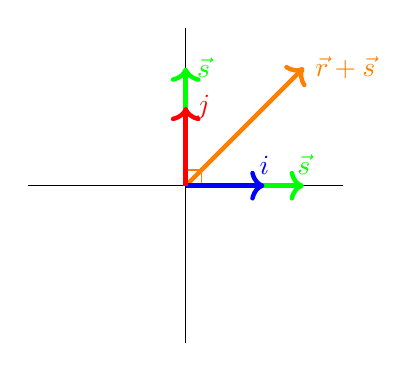
\begin{tikzpicture}
\coordinate (A) at (1, 0) {};
        \coordinate (B) at (0, 1) {};
        \coordinate (0) at (0, 0) {};

        \tkzMarkRightAngle[draw=orange,size=.2](A,0,B);    
    
\draw   (2,0) -- (-2, 0)
        (0,2) -- (0,-2);
\draw[->, ultra thick, green](0,0) -- (1.5,0)node (yaxis) [above] {$\vec s$} ;
\draw[->, ultra thick, green](0,0) -- (0,1.5)node (xaxis) [right] {$\vec s$};
\draw[->, ultra thick, orange](0,0) -- (1.5,1.5)node (xaxis) [right] {$\vec r + \vec s$};
\draw[->, ultra thick, blue](0,0) -- (1,0)node (yaxis) [above] {$i$} ;
\draw[->, ultra thick, red](0,0) -- (0,1)node (xaxis) [right] {$j$};
\end{tikzpicture}
\end{center}

\begin{center}
    \begin{tikzpicture}
\coordinate (A) at (1, 0) {};
        \coordinate (B) at (0, 1) {};
        \coordinate (0) at (0, 0) {};

        \tkzMarkRightAngle[draw=orange,size=.2](A,0,B);    
    
\draw   (2,0) -- (-2, 0)
        (0,2) -- (0,-2);
\draw[->, ultra thick, green](0,0) -- (1.5,0)node (yaxis) [below] {$\vec r$} ;
\draw[->, ultra thick, green](0,0) -- (0,1.5)node (xaxis) [left] {$\vec s$};

\draw[->, ultra thick, green](0,1.5) -- (1.5,1.5)node (yaxis) [above] {$\vec r$} ;
\draw[->, ultra thick, green](1.5,0)node (xaxis) [above] node(yaxis) [right]{$\vec s$} -- (1.5,1.5);
\draw[->, ultra thick, orange](0,0) -- (1.5,1.5)node (xaxis) [right] {$\vec r + \vec s$};
\draw[->, ultra thick, blue](0,0) -- (1,0)node (yaxis) [above] {$i$} ;
\draw[->, ultra thick, red](0,0) -- (0,1)node (xaxis) [right] {$j$};
\end{tikzpicture}
\end{flushright}

\end{center}


\subsection{Vector Multiplication}
\begin{flushleft}
\newline
In Vector Multiplication , we multiply a scalar value with a vector
\newline

In an example below 
$\vec r  = 
1.5 \times
\begin{bmatrix}
1\\
0
\end{bmatrix}
=
\begin{bmatrix}
1.5\\
0
\end{bmatrix}
$
$and$ $ \vec s = 
-1.5 \times
\begin{bmatrix}
0\\
$1$
\end{bmatrix}
=
\begin{bmatrix}
0\\
$-1.5$
\end{bmatrix}
$
\newline
Here, we multiplied scalar value of 1.5 to unit vector $\vec i$ and -1.5 to vector $\vec j$.

\begin{center}
    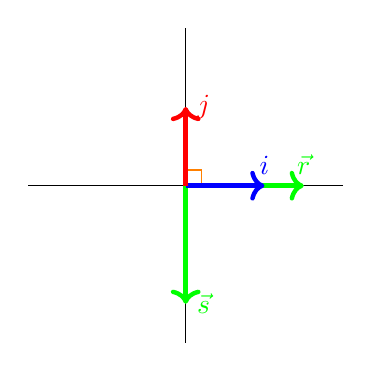
\begin{tikzpicture}
\coordinate (A) at (1, 0) {};
        \coordinate (B) at (0, 1) {};
        \coordinate (0) at (0, 0) {};

        \tkzMarkRightAngle[draw=orange,size=.2](A,0,B);    
    
\draw   (2,0) -- (-2, 0)
        (0,2) -- (0,-2);
\draw[->, ultra thick, green](0,0) -- (1.5,0)node (yaxis) [above] {$\vec r$} ;
\draw[->, ultra thick, green](0,0) -- (0,-1.5)node (xaxis) [right] {$\vec s$};
\draw[->, ultra thick, blue](0,0) -- (1,0)node (yaxis) [above] {$i$} ;
\draw[->, ultra thick, red](0,0) -- (0,1)node (xaxis) [right] {$j$};
\end{tikzpicture}
\end{center}
\end{flushleft}

\subsection{Vector Subtraction}
\begin{flushleft}
Vector Subtraction is addition of a vector having multiplied by -1 first.
\newline

$\vec r  = $
$
\begin{bmatrix}
$-2$\\
0
\end{bmatrix}
$
$and$ $ \vec s = $
$\begin{bmatrix}
0\\
$2$
\end{bmatrix}
$
\newline

therefore 
\newline

$\vec r - \vec s  = 
\begin{bmatrix}
$-2$\\
$0$
\end{bmatrix}
+(-1) \times
\begin{bmatrix}
$0$\\
$2$
\end{bmatrix}
=
\begin{bmatrix}
$-2$\\
$0$
\end{bmatrix}
+ 
\begin{bmatrix}
$0$\\
$-2$
\end{bmatrix}
=
\begin{bmatrix}
$-2$\\
$-2$
\end{bmatrix}
$
\newline

Here $\vec s$ is first multiplied by -1 and then added with $\vec r$.

\begin{center}
    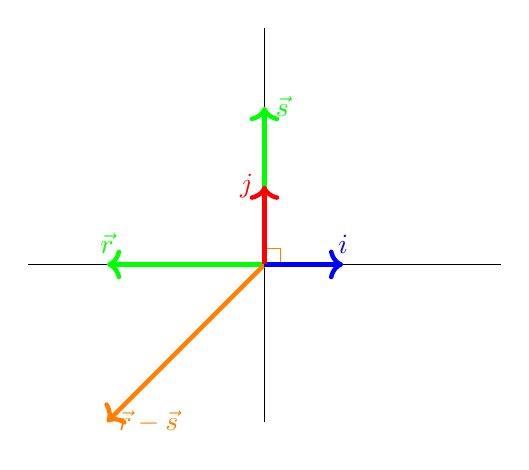
\begin{tikzpicture}
\coordinate (A) at (1, 0) {};
        \coordinate (B) at (0, 1) {};
        \coordinate (0) at (0, 0) {};

        \tkzMarkRightAngle[draw=orange,size=.2](A,0,B);    
    
\draw   (3,0) -- (-3, 0)
        (0,3) -- (0,-2);
\draw[->, ultra thick, green](0,0) -- (-2,0)node (yaxis) [above] {$\vec r$} ;
\draw[->, ultra thick, green](0,0) -- (0,2)node (xaxis) [right] {$\vec s$};
\draw[->, ultra thick, orange](0,0) -- (-2,-2)node (xaxis) [right] {$\vec r - \vec s$};
\draw[->, ultra thick, blue](0,0) -- (1,0)node (yaxis) [above] {$i$} ;
\draw[->, ultra thick, red](0,0) -- (0,1)node (xaxis) [left] {$j$};
\end{tikzpicture}
\end{center}
\end{flushleft}

\section{Modulus and Inner product}
\begin{flushleft}
The magnitude is also called the modulus or the length of the vector.
\newline
For Example, modulus of a vector $\vec r$ = $ a \vec i + b \vec j$ =
$
\begin{bmatrix}
$a$\\
b
\end{bmatrix}
$
is given as, 
\newline

$|\vec r|$ = $\sqrt{a^2 + b^2}$

\begin{center}
    \begin{tikzpicture}
\coordinate (A) at (1, 0) {};
        \coordinate (B) at (0, 1) {};
        \coordinate (0) at (0, 0) {};

        \tkzMarkRightAngle[draw=orange,size=.2](A,0,B);    
    
\draw   (2,0) -- (-2, 0)
        (0,2) -- (0,-2);
\draw[->, ultra thick, green](0,0) -- (1.5,0)node (yaxis) [below] {$\vec a\vec i$ $|\vec a|$} ;

\draw[->, ultra thick, green](1.5,0) node (xaxis) [right] node(yaxis) [above]{$b\vec j$ $|\vec b|$} -- (1.5,1.5);
\draw[->, ultra thick, orange](0,0) -- (1.5,1.5)node (yaxis) [above] {$|\vec r|$ = $\sqrt{a^2 + b^2}$};

\draw[->, ultra thick, blue](0,0) -- (1,0)node (yaxis) [above] {$i$} ;
\draw[->, ultra thick, red](0,0) -- (0,1)node (xaxis) [right] {$j$};

\end{tikzpicture}
\end{center}

\newline
Inner product of vectors is multiplication of each component of vectors then addition of the multiplied product giving a scalar result.

\begin{center}
    \begin{tikzpicture}
\coordinate (A) at (1, 0) {};
        \coordinate (B) at (0, 1) {};
        \coordinate (0) at (0, 0) {};

        \tkzMarkRightAngle[draw=orange,size=.2](A,0,B);    
    
\draw   (2,0) -- (-2, 0)
        (0,2) -- (0,-2);
\draw[->, ultra thick, green](0,0) -- (3,2)node (yaxis) [below] {$\vec \vec r$ = $
\begin{bmatrix}
$3$\\
2
\end{bmatrix}
$} ;
\draw[->, ultra thick, green](0,0) node (xaxis) [left] node(yaxis) [below]{$\vec s$ = $
\begin{bmatrix}
$-1$\\
2
\end{bmatrix}
$} -- (-1,2);

\draw[->, ultra thick, blue](0,0) -- (1,0)node (yaxis) [above] {$i$} ;
\draw[->, ultra thick, red](0,0) -- (0,1)node (xaxis) [right] {$j$};

\end{tikzpicture}
\end{center}

\subsection{Commutative Property}
Inner product or Dot product follows commutative property.
\newline

$\vec r \cdot \vec s$
\newline
= r_is_i + r_js_j
\newline
= 3\cdot -1 + 2 \cdot 2
\newline
= -3 + 4 = 1
\newline
= s \cdot r

\subsection{Distributive over Addition}

r\cdot(s + t) = r\cdot s + r\cdot t
\newline

$
r =
\begin{bmatrix}
r_1\\
r_2\\
.\\
.\\
r_n
\end{bmatrix}
$
,
$
s =
\begin{bmatrix}
s_1\\
s_2\\
.\\
.\\
s_n
\end{bmatrix}
$
,
$
t =
\begin{bmatrix}
t_1\\
t_2\\
.\\
.\\
t_n
\end{bmatrix}
$
\newline

r\cdot(s + t) 
\newline
= r_1\cdot(s_1 + t_1) + r_2\cdot(s_2 + t_2) + ... + r_n\cdot(s_n + t_n)
\newline
= r_1\cdot s_1 + r_1\cdot t_1 + r_2\cdot s_2 + r_2\cdot t_2 + ... + r_n\cdot s_n + r_n\cdot t_n
\newline
= (r_1\cdot s_1 + r_2\cdot s_2 + ... + r_n\cdot s_n) + (r_1\cdot t_1 + r_2\cdot t_2 + ... + r_n\cdot t_n)
\newline
= r\cdot s + r\cdot t
\newline


Hence Proved

\subsection{Associative over Scalar Multiplication}
r\cdot(a\cdot s) = a\cdot(r\cdot s)
\newline
\newline
LHS = r_1\cdot(a_1\cdot s_1) + r_2\cdot(a_2\cdot s_2)
\newline
= a\cdot(r_1\cdot s_1 + r_2\cdot s_2)
\newline
= a\cdot(r\cdot s)
\newline

Hence Proved

\end{flushleft}


\section{Cosine and Dot Product}
\begin{flushleft}

\begin{center}
    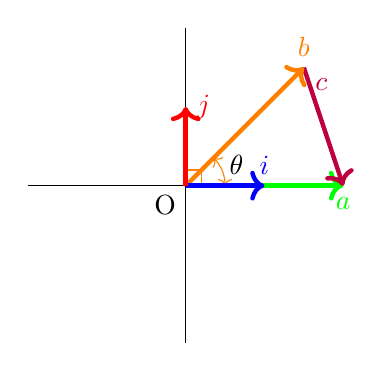
\begin{tikzpicture}
\coordinate (A) at (1, 0) {};
        \coordinate (B) at (0, 1) {};
        \coordinate (0) at (0, 0) {};

        \tkzMarkRightAngle[draw=orange,size=.2](A,0,B);    
    
\draw
    (2,0) coordinate (a) 
    -- (0,0) coordinate (O) node[below left] {O}
    -- (1.5,1.5) coordinate (c) 
    pic["$\theta$", draw=orange, <->, angle eccentricity=1.4, angle radius=0.5cm]
    {angle=a--O--c};    
    
  
    
\draw   (2,0) -- (-2, 0)
        (0,2) -- (0,-2);
\draw[->, ultra thick, green](0,0) -- (2,0)  node[below] {$a$} ;

\draw[->, ultra thick, purple](1.5,1.5)  node[below right]{$c$} -- (2,0);
\draw[->, ultra thick, orange](0,0) -- (1.5,1.5)node (yaxis) [above] {$b$};


\draw[->, ultra thick, blue](0,0) -- (1,0)node (yaxis) [above] {$i$} ;
\draw[->, ultra thick, red](0,0) -- (0,1)node (xaxis) [right] {$j$};





\end{tikzpicture}
\end{center}

We know that by Cosine Rule,
\newline

c^2 = a^2 + b^2 - 2ab \cos \theta
\newline

 $\therefore |\vec r - \vec s| = |\vec r| + |\vec s| - 2|\vec r||\vec s| \cos \theta$
\newline

$= (\vec r - \vec s)\cdot (\vec r - \vec s) =\vec r \cdot \vec r - \vec s \cdot \vec r - \vec s \cdot \vec r - \vec s \cdot \vec s$
\newline

$= |\vec{r} ^2| - 2 \vec s \cdot \vec r + |\vec s^2|$
\newline

Now by Equation (1) and (2),
\newline

$\implies \vec s \cdot \vec r = - 2|\vec r||\vec s|\cos \theta$
\newline
\newline
$\therefore \fcolorbox{black}{gray!30}{$\vec r \cdot \vec s = |\vec r||\vec s|\cos \theta$}$
\newline
\newline
Examples,
\newline


\begin{center}
    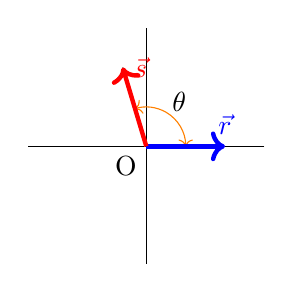
\begin{tikzpicture}
    
\draw   (1.5,0) -- (-1.5, 0)
        (0,1.5) -- (0,-1.5);
        
\draw
    (1,0) coordinate (a) 
    -- (0,0) coordinate (O) node[below left] {O}
    -- (-0.3,1) coordinate (c) 
    pic["$\theta$", draw=orange, <->, angle eccentricity=1.4, angle radius=0.5cm]
    {angle=a--O--c};           

\draw[->, ultra thick, blue](0,0) -- (1,0)node (yaxis) [above] {$\vec r$} ;
\draw[->, ultra thick, red](0,0) -- (-0.3,1)node (xaxis) [right] {$\vec s$};
\end{tikzpicture}
\end{center}
But when $\theta = 90\si{\degree},$ $\cos 90\si{\degree} = 0, \therefore \vec r \cdot \vec s = 0$
\newline

Also when $\theta = 180\si{\degree},$ $\cos 180\si{\degree} = -1, \therefore \vec r \cdot \vec s = -|\vec r||\vec s|$
\newline

And when $\theta = 0\si{\degree},$ $\cos 0\si{\degree} = 1, \therefore \vec r \cdot \vec s = |\vec r||\vec s|$

\end{flushleft}

\section{Projection of Vectors}

\begin{center}
    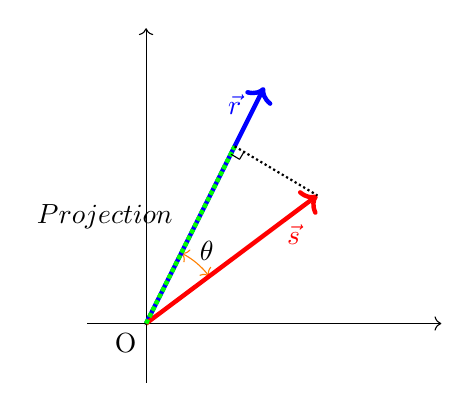
\begin{tikzpicture}[scale=0.75]

\draw
    (2.9,2.17) coordinate (a) 
    -- (0,0) coordinate (O) node[below left] {O}
    -- (1.5,3) coordinate (c) 
    pic["$\theta$", draw=orange, <->, angle eccentricity=1.2, angle radius=1cm]
    {angle=a--O--c};
    
\draw[->] (-1,0) -- (5,0);
\draw[->] (0,-1) -- (0,5);
\draw[->,ultra thick, blue] (0,0) -- (2,4);
\draw[->,ultra thick, red] (0,0) -- (2.9,2.17);
\draw[densely dotted, ultra thick, green] (0,0) -- (1.5,3);
\draw[densely dotted, thick] (1.5,3) -- (2.9,2.17);
\draw [blue](1.5,3.7) node {$\ul{\vec r}$};
\draw [red](2.5,1.5) node {$\ul{\vec s}$};
\draw (-0.7,1.8) node {$\ul{Projection}$};
\draw[yshift=73,xshift=35,scale=0.1] (2.1,3) -- (3.5,2.17);
\draw[yshift=73,xshift=53.5,scale=0.1,rotate=90] (2.1,3) -- (3.5,2.17);
    
    
\end{tikzpicture}
\end{center}

\begin{flushleft}


\cos \theta = \frac{Adjacent}{Hypotenuse} = \frac{Adjacent}{|\vec s|}
\newline

$\therefore \vec r \cdot \vec s = |\vec r||s|\cos \theta$
\newline
Where \rightarrow |s|\cos \theta
\newline

$\therefore \vec r \cdot \vec s = |\vec r|\cdot$ Projection
\newline

\textit{\textbf{Scalar Projection}} \rightarrow \frac{\vec r \cdot \vec s}{|\vec r|} = |\vec s|\cdot \cos \theta
\newline

\textit{\textbf{Vector Projection}} \rightarrow \frac{\vec r \cdot \vec s \cdot \vec r}{|\vec r|\cdot |\vec r|} 
\newline

\end{flushleft}



\begin{minipage}[b]{0.4\linewidth}
\section*{It's Testing Time}
\newline
\end{minipage}
\hfill
\begin{minipage}[b]{0.6\linewidth}

\includegraphics[height=3\baselineskip]{testing_time.jpg}
\end{minipage}
\begin{flushleft}
\begin{enumerate}
    \item A ship travels with velocity given by $
\begin{bmatrix}
1\\
2
\end{bmatrix}
$, with current flowing in the direction given by $
\begin{bmatrix}
1\\
1
\end{bmatrix}
$ with respect to some co-ordinate axes.
\newline

What is the velocity of the ship in the direction of the current?
\newline
\textit{(Hint: Apply Projection that you have studied now)}

\item At 12:00 pm, a spaceship is at position $
\begin{bmatrix}
3\\
2\\
4
\end{bmatrix}
$km away from the origin with respect to some 3 dimensional co ordinate system. The ship is travelling with velocity $
\begin{bmatrix}
-1\\
2\\
-3
\end{bmatrix}
$km/h What is the location of the spaceship after 2 hours have passed?
\newline


\end{enumerate}


\textit{\textbf{Note:} Solutions are given at the end of the document.}

\end{flushleft}

\section{Linear Dependence and Independence}
\begin{flushleft}

\subsection{What are Linear Dependence and Independence?}
\textbf{Linear Dependence} in a system of linear equations having more than or two equations referring to the same line containing infinite number of solutions to satisfy the conditions of the equations.
\newline
\newline

\textbf{Linear Independence} in system of linear equations means that the two equations only meet at one point i.e.(the intersection between the two lines). This single point in the entire universe will solve both equations at the same time. 
\newline
\newline

\textbf{Testing Equations for Dependence and Independence:}

\begin{enumerate}
    \item If the slopes are different, then the system is independent.
    \item If the slopes are the same, then the system is either dependent (same line) or inconsistent (parallel lines).
\end{enumerate}

\begin{center}
    \includegraphics[width=12cm,height=4.2cm]{"sys".jpg}
\end{center}

\subsection{Linearly Dependent Vectors}
Vectors are linearly dependent if there is a linear combination of them that equals the zero vector, without the coefficients of the linear combination being zero.
\[ a_1\vec v_1 + a_3\vec v_2 + ... + a_n\vec v_n = \vec 0\]

\subsection{Linearly Independent Vectors}
Several vectors are linearly independent if none of them can be expressed as a linear combination of the others.
\[ a_1\vec v_1 + a_3\vec v_2 + ... + a_n\vec v_n = \vec 0\]
\[a_1 = a_2 = ... = a_n = 0\]





\end{flushleft}



\section{Basis}
\begin{flushleft}
Basis is a set of n vectors that:
\begin{enumerate}
    \item Are not linear combinations of each others(Linearly Independent).
    \item Span the space
    \newline
    The Space is then n dimensional. 
\end{enumerate}

\begin{center}
    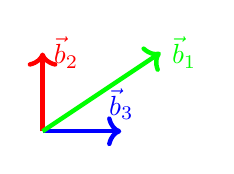
\begin{tikzpicture}
    
\draw[->, ultra thick, blue](0,0) -- (1,0)node (yaxis) [above] {$\vec b_3$};
\draw[->, ultra thick, red](0,0) -- (0,1)node (xaxis) [right] {$\vec b_2$};
\draw[->, ultra thick, green](0,0) -- (1.5,1)node (xaxis) [right] {$\vec b_1$};
\end{tikzpicture}
\end{center}

Here $\vec b_3$ \ne $a_1\vec b_1$ + $a_2\vec b_2$ \rightarrow \textit{Linearly Independent}
\end{flushleft}

\section{Matrices}
\subsection{What are Matrices?}
\begin{flushleft}
A Matrix is a rectangular array of numbers arranged in rows and columns. 
\newline
For Example:
\begin{center}
    \begin{bmatrix}
a_{11} & a_{12} & a_{13} & a_{14}\\
a_{21} & a_{22} & a_{23} & a_{34}\\
a_{31} & a_{32} & a_{33} & a_{34}\\
\end{bmatrix}
\end{center}
The number of rows and columns that a matrix has is called its \textbf{dimension} or its \textbf{order}. The dimension (or order) of the above matrix is 3 x 4, meaning that it has 3 rows and 4 columns.
\newline
Numbers that appear in the rows and columns of a matrix are called \textbf{elements} of the matrix.
\newline

\textbf{Matrices can be used to solve Simultaneous Equations.}

In the above apples and bananas problem, we have transformed a equation into the matrix form.
\begin{equation*}
    3a+1b = 10,  1a + 1b = 4
\end{equation*}

\begin{center}
    \begin{bmatrix}
3 & 1\\
1 & 1 
\end{bmatrix}
\begin{bmatrix}
a\\
b
\end{bmatrix}
=
\begin{bmatrix}
10\\
4
\end{bmatrix}
\end{center}

\textbf{Matrices can also be used to transform Space.}


The above matrix form can be represented as:
\begin{center}
    $A\cdot r = r^'$

    $A \cdot nr = r^'$
    
\fcolorbox{black}{gray!30}{$Where,  A \rightarrow Matrix,
r \rightarrow  $Original Vector,$
$ r' \rightarrow$ Spanned Vector}
\end{center}



\begin{center}
    $A\cdot (n \vec e_1 + n \vec e_2) = n A \vec e_1 + n A \vec e_2$
    \newline
    
    
    \fcolorbox{black}{gray!30}{Where,  $ \vec e_1, \vec e_2 \rightarrow$ Unit Vector along X axis and Y axis respectively}
\end{center}

Let us take a vector $r=
\begin{bmatrix}
 3\\
 2
\end{bmatrix}$
and span it using matrix $A =
\begin{bmatrix}
2 & 3\\
10 & 1
\end{bmatrix}
$ 

\begin{center}
$\therefore$
    \begin{bmatrix}
2 & 3\\
10 & 1 
\end{bmatrix}
\begin{bmatrix}
3\\
2
\end{bmatrix}
\end{center}


\end{flushleft}

\begin{center}
$\therefore$
\begin{bmatrix}
2 & 3\\
10 & 1 
\end{bmatrix}
 $\Bigg( 3*$
\begin{bmatrix}
1\\
0
\end{bmatrix}
$+ 2*$
\begin{bmatrix}
0\\
1
\end{bmatrix}
\Bigg)
$ = $
\begin{bmatrix}
12\\
32
\end{bmatrix}
\end{center}

The Vector $\begin{bmatrix}
3\\
2
\end{bmatrix}$ is spanned into \begin{bmatrix}
12\\
32
\end{bmatrix}

\subsection{Matrix Transformation}
\begin{flushleft}
Let us apply Transformation Matrix $\begin{bmatrix}
-1&0\\
0&2
\end{bmatrix}$ to unit vectors $\vec e_1$ and $\vec e_2$.

\begin{center}
    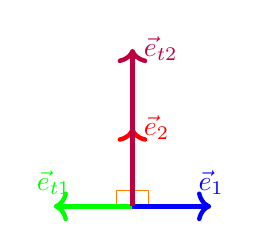
\begin{tikzpicture}
\coordinate (A) at (1, 0) {};
        \coordinate (B) at (0, 1) {};
        \coordinate (0) at (0, 0) {};
         \coordinate (C) at (-1, 0) {};

        \tkzMarkRightAngle[draw=orange,size=.2](A,0,B);   
        \tkzMarkRightAngle[draw=orange,size=.2](B,0,C);
    
\draw[->, ultra thick, blue](0,0) -- (1,0)node (yaxis) [above] {$\vec e_1$};
\draw[->, ultra thick, red](0,0) -- (0,1)node (xaxis) [right] {$\vec e_2$};
\draw[->, ultra thick, green](0,0) -- (-1,0)node (xaxis) [above] {$\vec e_{t1}$};
\draw[->, ultra thick, purple](0,0) -- (0,2)node (xaxis) [right] {$\vec e_{t2}$};
\end{tikzpicture}
\newline

\fcolorbox{black}{gray!30}{Where,  $ \vec e_{t1}, \vec e_{t2} \rightarrow$ Vector Transformed from $\vec e_1,$ $ \vec e_2$ respectively}
\end{center}

These matrices can also be used to rotate the vectors along the plane.
\newline
For Example using,
\begin{center}
   \begin{bmatrix}
\cos \theta & \sin \theta\\
-\sin \theta & \cos \theta 
\end{bmatrix} 
\end{center}
and other matrices.
\end{flushleft}

\subsection{Composition or Combination}
\begin{flushleft}
We can apply n transformations to a vector by combining these transformation matrix. 
\newline
But the order in which we apply this transformation can also change the results.
\newline
For Example, Let us take two transformation matrix A_1 = $\begin{bmatrix}
0&1\\
-1&0
\end{bmatrix} and A_2 = \begin{bmatrix}
-1&0\\
0&1
\end{bmatrix}.$
\newline
Now,
A_1\cdot A_2 = $\begin{bmatrix}
0&1\\
-1&0
\end{bmatrix} and $
A_2\cdot A_1 = $\begin{bmatrix}
0&-1\\
-1&0
\end{bmatrix}$
\newline

From above we can conclude that,
\begin{center}
    \fcolorbox{black}{gray!30}{$A_1\cdot A_2 \ne A_2\cdot A_1$}

\end{center}
\end{flushleft}

\subsection{Determinant and Inverse}
\begin{flushleft}
A determinant of a matrix represents a single number which is obtained by multiplying and adding its elements in a special way.

Determinant of 2 x 2 Matrix:
\newline

 $A = \begin{bmatrix} a & b\\  c & d \end{bmatrix},  \begin{vmatrix} A \end{vmatrix}= ad - bc$ 
\newline

Determinant of 3 x 3 Matrix:
\newline

 $A = \begin{bmatrix} a & b & c\\  d & e & f\\  g & h & i \end{bmatrix}  \begin{vmatrix} A \end{vmatrix}= a(ei-fh)-b(di-gf)+c(dh-eg)$
 \newline

For example, if we have the 2 $\times$ 2 square matrix:

\begin{center}
    $\begin{bmatrix}{5}&{7}\\{2}&-{3}\end{bmatrix}$
\end{center}
\newline

then the determinant of this matrix is written within vertical lines as follows:
\begin{center}
    $\displaystyle{\left|\begin{matrix}{5}&{7}\\{2}&-{3}\end{matrix}\right|} = [(5)(3)+(7)(2)] = 29$
\end{center}
\newline


The inverse of a square matrix A, sometimes called a reciprocal matrix, is a matrix $A^{\mbox{-}1}$ such that

  $A A^{\mbox{-}1}=I,$ 	
  
where I is the identity matrix. 
\newline


A square matrix A has an inverse if the determinant $|A|! = 0$ . A matrix possessing an inverse is called non singular or invertible otherwise, matrix is a singular matrix.
\newline

For  $2 \times 2$ matrix, 
\newline

 $ A = \begin{bmatrix}
 a & b\\
 c & d
 \end{bmatrix}$
\newline

it's inverse is given as,
\newline

$A^{\mbox{-}1}	=	1/(\textvert{}A\textvert{})  \begin{bmatrix}
 d & -b\\
 -c & a
 \end{bmatrix}	
	=	1/(ad-bc)\begin{bmatrix}
 d & -b\\
 -c & a
 \end{bmatrix}	$
\newline 

A general n $\times$ n matrix can be inverted using methods such as the Gauss-Jordan elimination, Gaussian elimination or LU decomposition.



\end{flushleft}

\section{Solving using Elimination}
\begin{flushleft}
For solving equation in matrix form, we have to reduce matrix.
\newline
There are various methods for reducing the matrices, some of theme are:
\subsection{Echelon Method}
In this method, the given matrix is reduced into echelon form.
\newline
Echelon form of any matrix is the one having following properties:
\begin{enumerate}
    \item All zero rows (if any) belong at the bottom of the matrix.
    \item A pivot in a non-zero row, which is the left-most non-zero value in the row, is always strictly to the right of the pivot of the row above it.
\end{enumerate}
\newline
    For Example,
\begin{center}
    $\begin{bmatrix}
1 & 2 & 5 & 8\\
0 & 6 & 3 & 9\\
0 & 0 & 0 & 1\\
0 & 0 & 0 & 0
\end{bmatrix}
,
\begin{bmatrix}
1 & 2 & 5 \\
0 & 6 & 3 \\
0 & 0 & 1
\end{bmatrix}
, etc$
\end{center}
\end{flushleft}

\subsection{Gauss Elimination}
\begin{flushleft}
Important Conclusion:
\fcolorbox{black}{gray!30}{$A\cdot A^{\mbox{-}1} = I$}
\newline

In Gauss Elimination, we reduce the $n\times n$ matrix into Identity matrix to solve the simultaneous equation or get the values of elements in the vector. 

For Example
\newline

$\begin{bmatrix}
1 & 2 & 5 \\
0 & 6 & 3 \\
0 & 0 & 1
\end{bmatrix} 
\begin{bmatrix}
a \\
b \\
c
\end{bmatrix} = 
\begin{bmatrix}
15\\
10\\
5
\end{bmatrix}$
\newline

We can represent the above expression as,
\newline
$AX = B$
    \newline
    Multiplying Both sides by $A^{\mbox{-} 1}$$, we get
    \newline
    $$\therefore  A^{\mbox{-} 1}AX = A^{\mbox{-}1}B$
    \newline
    $\therefore IX = A^{\mbox{-}1}B$
    \newline
    
 \fcolorbox{black}{gray!30}{$X = A^{\mbox{-}1}B $}
\end{flushleft}

\section{Einstein Summation Convention}
\begin{flushleft}
Einstein summation convention is a notational convention that implies summation over a set of indexed terms in a formula.
\newline

Suppose we have to multiple two matrices
\newline

$A = \begin{bmatrix}
a_{11} & a_{12} & a_{13} & ... & a_{14}\\
a_{21} & a_{22} & a_{23} & ... & a_{34}\\
: & : & : & ... & :\\
: & : & : & ... & :\\
a_{n1} & a_{n2} & a_{n3} & ... & a_{n4}
\end{bmatrix} and  B = \begin{bmatrix}
b_{11} & b_{12} & b_{13} & ... & b_{14}\\
b_{21} & b_{22} & b_{23} & ... & b_{34}\\
: & : & : & ... & :\\
: & : & : & ... & :\\
b_{n1} & b_{n2} & b_{n3} & ... & b_{n4}
\newline
\end{bmatrix}$

to give matrix AB.

If we want element $ab_{13}$ of matrix AB, we have to do,

$ab_{13} = a_{11}b_{13} + a_{12}b_{23} + ... + a_{1n}b_{n3}$
\newline

Now Einstein Summation Convention says that, the element can be found using the expression,
\newline

$\therefore$\fcolorbox{black}{gray!30}{$ab_{ik} = \sum\limits_{j=1}^n a_{ij}b_{jk} = a_{ij}b_{jk}$} 
\newline

If we do this for all the possible cases of i and k we get the entire AB matrix.
\end{flushleft}





\newpage
\section{Solutions}
\begin{flushleft}
\begin{enumerate}
    \item Since the problem is using velocity as a vector. We want the projection of the ship velocity onto the current velocity. 
\newline

    Let u = $
\begin{bmatrix}
1\\
2
\end{bmatrix}$ be the vector representing the ship's velocity and v = $
\begin{bmatrix}
1\\
1
\end{bmatrix}$  be the vector representing current direction.
\newline    
\therefore v\cdot \frac{u\cdot v}{|v|^2} = $
\begin{bmatrix}
1.5\\
1.5
\end{bmatrix}

\item Initial position of the Spaceship was
$
\begin{bmatrix}
3\\
2\\
4
\end{bmatrix}
$km
\newline
 It's velocity is
$
\begin{bmatrix}
-1\\
2\\
-3
\end{bmatrix}
$km/h 

So, in 2 hours, it travels $ 2 *
\begin{bmatrix}
-1\\
2\\
-3
\end{bmatrix}
$kms respectively in 3D co-ordinate system.
\newline

Then it's final position willl be:
\newline

$
\begin{bmatrix}
3\\
2\\
4
\end{bmatrix}
 + $
 $
\begin{bmatrix}
-2\\
4\\
-6
\end{bmatrix}
 = $
$
\begin{bmatrix}
1\\
6\\
2
\end{bmatrix}
 km$



\end{enumerate}
\end{flushleft}



\end{document}


